\documentclass[11pt]{article}

%%%%%%%%%%%%%%Include Packages%%%%%%%%%%%%%%%%%%%%%%%%%%
\usepackage{xcolor}
\usepackage{mathtools}
\usepackage[a4paper, total={6in, 8in}, margin=1.25in]{geometry}
\usepackage{amsmath}
\usepackage{amssymb}
\usepackage{paralist}
\usepackage{rsfso}
\usepackage{amsthm}
\usepackage{wasysym}
\usepackage[inline]{enumitem}   
\usepackage{hyperref}
\usepackage{tocloft}
\usepackage{titlesec}
\usepackage{colortbl}
\usepackage{wrapfig}
\usepackage{pdfpages}
\usepackage[american]{circuitikz}
%%%%%%%%%%%%%%%%%%%%%%%%%%%%%%%%%%%%%%%%%%%%%%%%%%%%%%%%



\begin{document}
\Large \noindent \textbf{Physics 5C Discussion (Worksheet 8)}\\
\normalsize
Department of Physics and Astronomy, UCLA\\

\noindent TA: Jinyan Miao (jnmiu@ucla.edu)\\
Office hours: Thursday 2:30 - 4:30 PM (PST) over Zoom \\
Zoom ID: 963 5916 9873 (passcode: hiJinyan)\\
Click for the \href{https://ucla.zoom.us/j/96359169873?pwd=05p7ssCPwTbl8KfxoBNCOuaIbt68jW.1}{\underline{Zoom link}} and \href{https://sites.google.com/umich.edu/jmiu/worksheets}{\underline{solutions to the worksheets}}.\\
\noindent\rule{8cm}{0.4pt}\\

\noindent\textbf{Problem 1}: Jinyan is doing some weird experiment again: He builds a circuit and places two straight wires close to each other as shown. Then he sees that the two wires repel each other. Please educate him on how to write his lab report.
\begin{center}
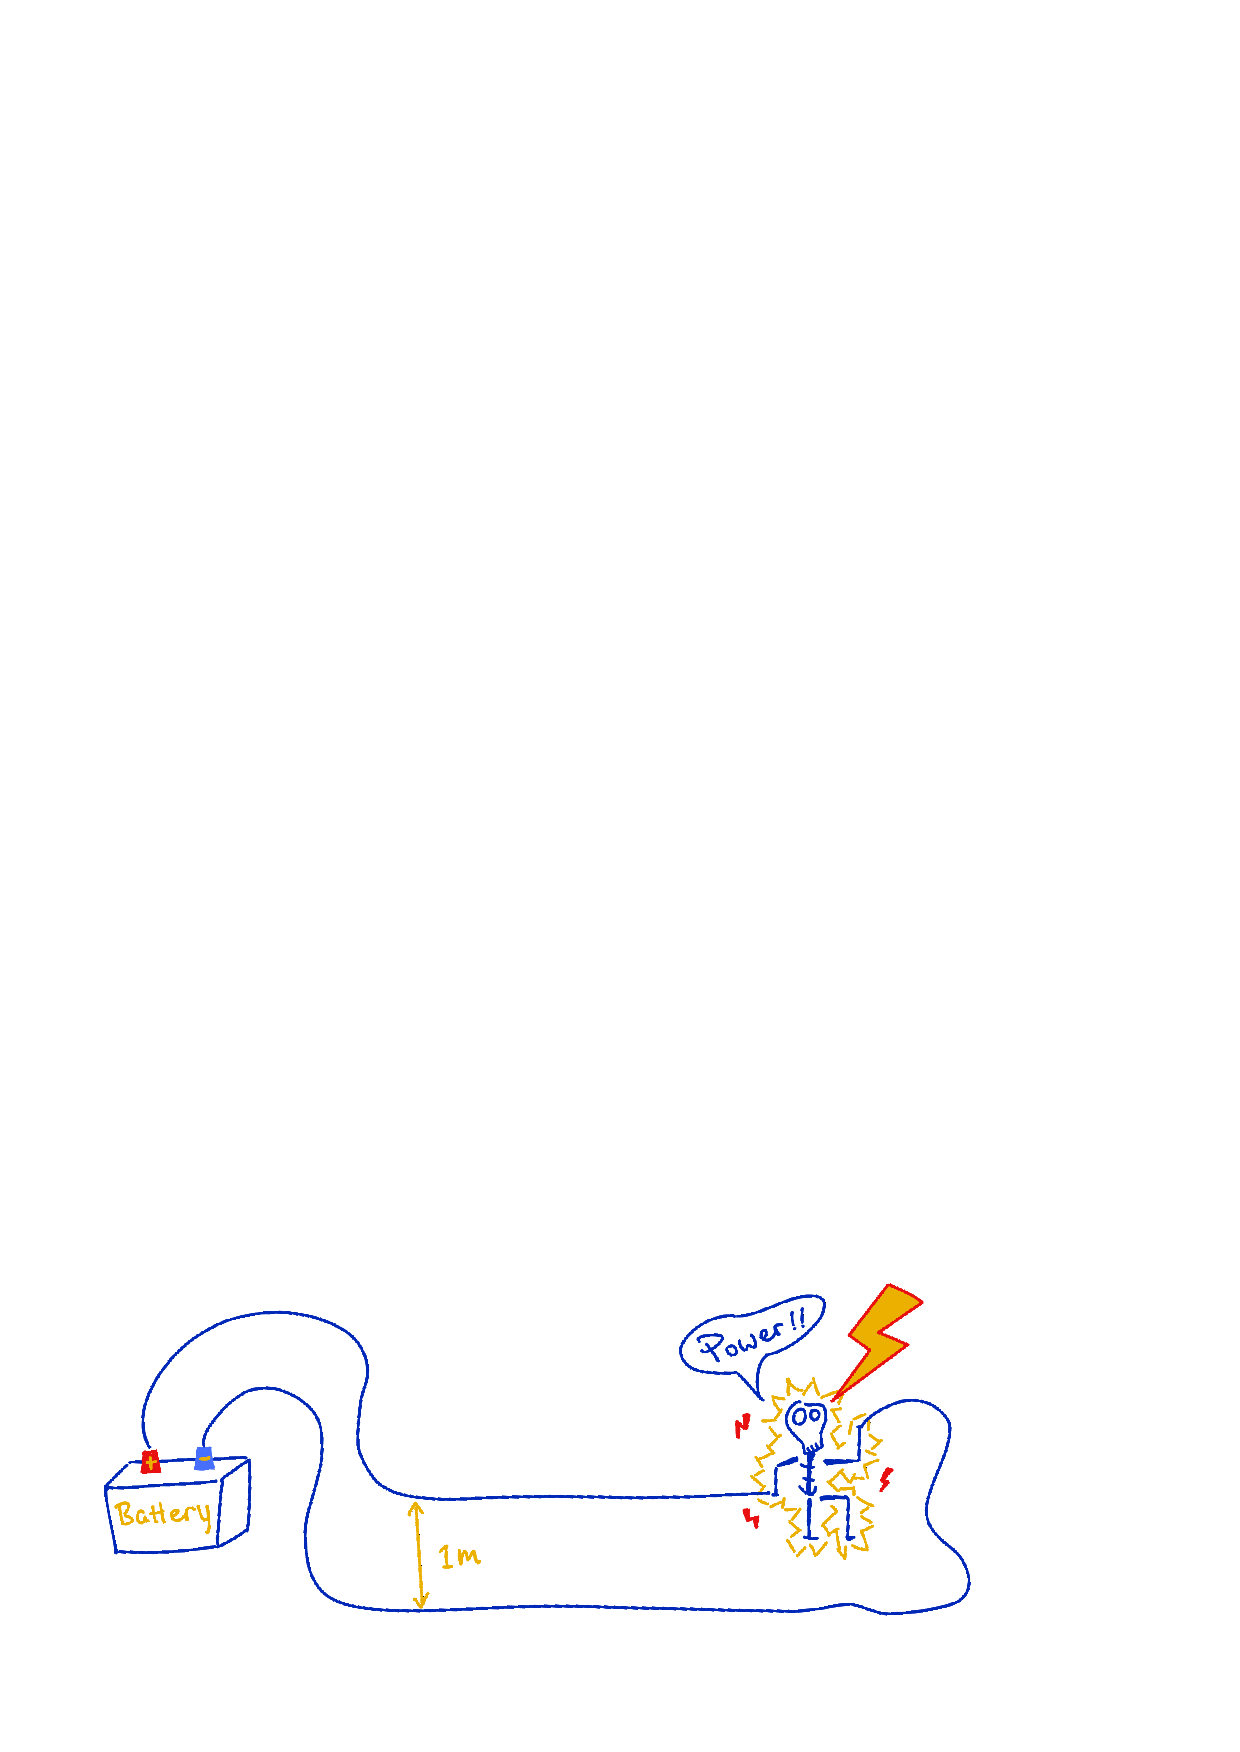
\includegraphics[scale=0.85]{parallelWires}
\end{center}
\noindent \textbf{Part (a)} In what direction are the electrons in the wires moving?\\

\noindent \textbf{Part (b)} Why do the two wires repel each other?\\

\noindent \textbf{Part (c)} If the current in the wire is $50$\,$\mu$A, the distance between the two wires is $1\,\text{m}$, and an electron in the top wire is moving $1\,\text{nm/s}$, what is the repelling force experienced by the electron? Include both direction and magnitude in your answer.\\


\newpage
\noindent \textbf{Problem 2}: Current produces a magnetic field. \\

\begin{wrapfigure}[10]{r}{0.55\textwidth}
  \begin{center}
  \vspace{-29pt}
    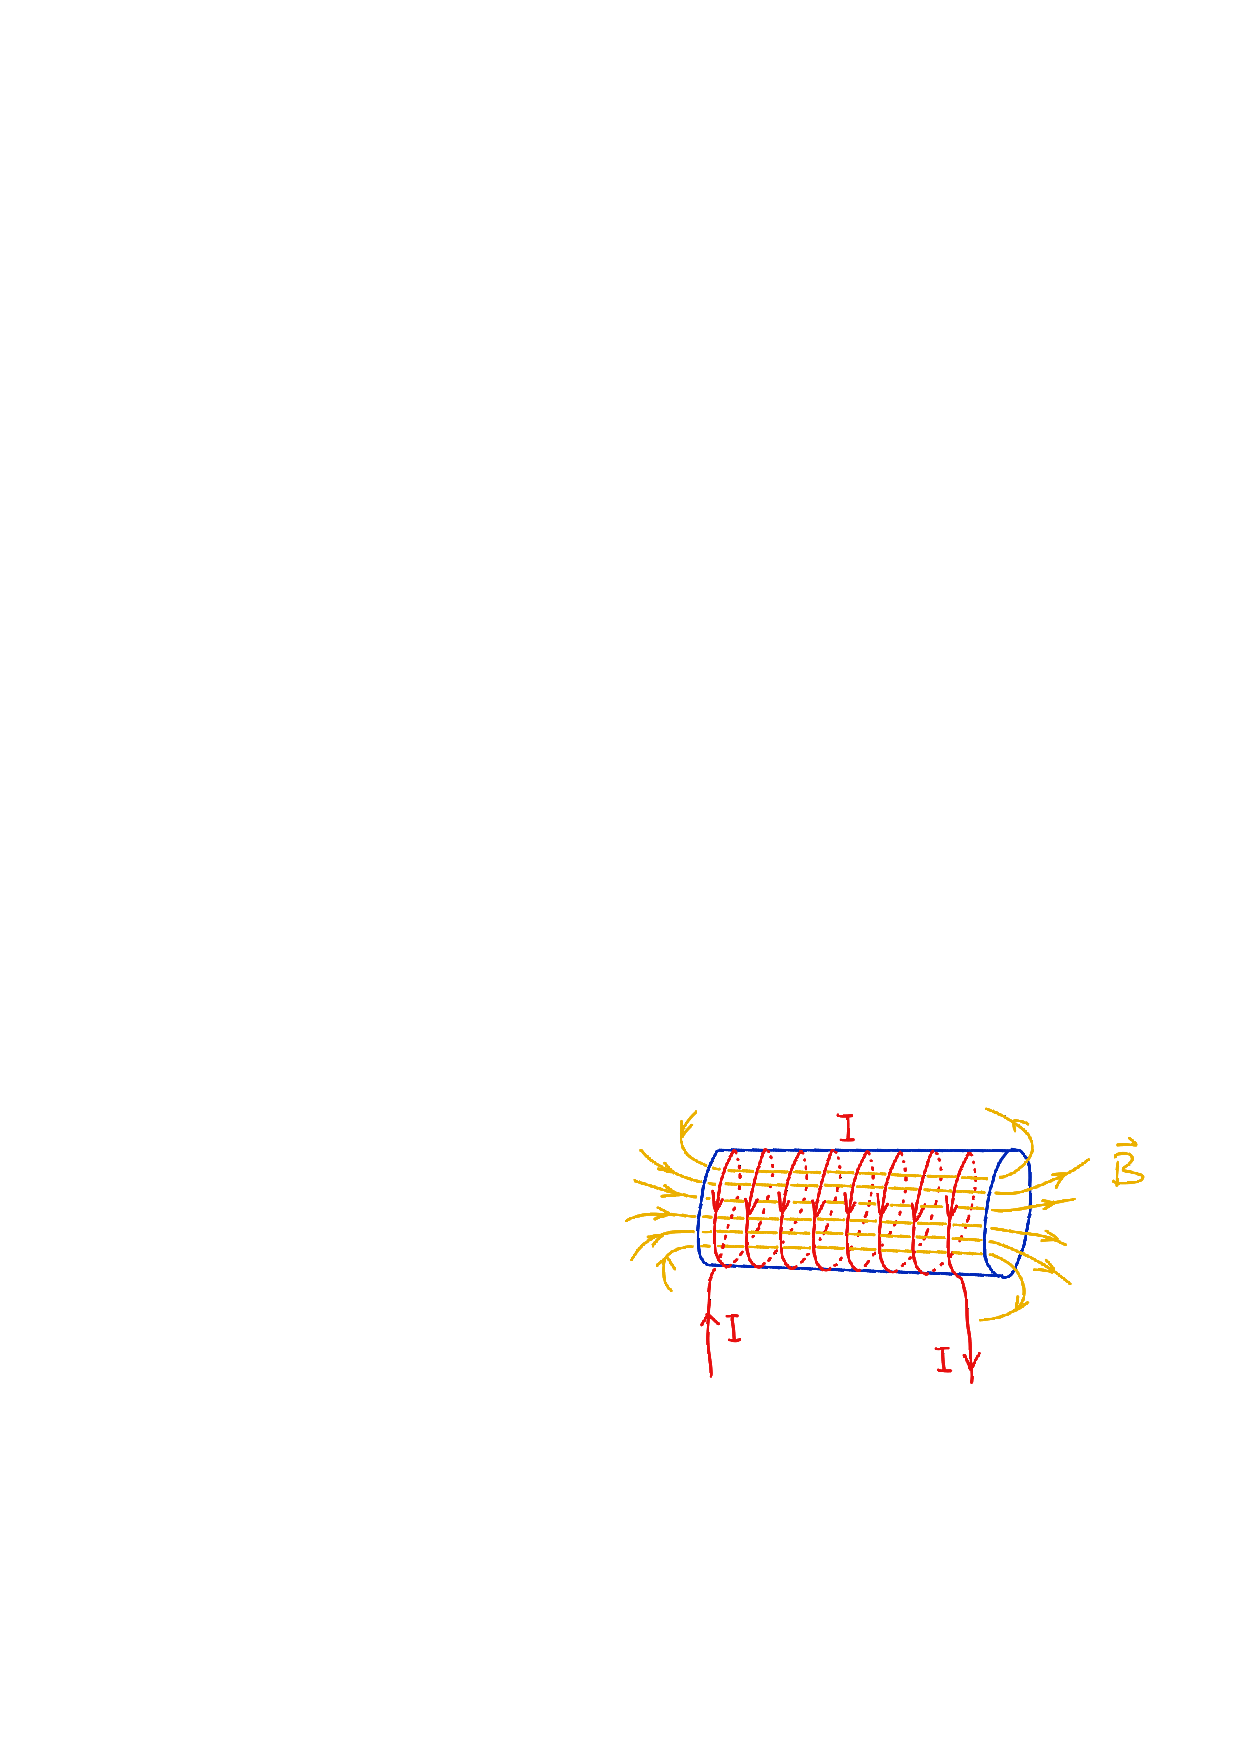
\includegraphics[scale=0.85]{solenoid}
  \end{center}
\end{wrapfigure}

\noindent If we wind the wire into a solenoid, the magnetic field inside the solenoid produced by the current is uniform, 
\begin{align*}
|\vec{B}| = \mu_0 N I/L \,,
\end{align*}
where $\mu_0$ is a constant, $N$ is the number of ``wire loops," $I$ is the current in the wire, and $L$ is the solenoid length. The direction of $\vec{B}$ is determined by the right-hand rule. \\

\noindent \textbf{Part (a)} Explain why the magnetic field inside a long (but has a finite length) solenoid is stronger and more uniform than the field outside.\\

\noindent \textbf{Part (b)} Jinyan needs a $1\,$T magnetic field for his science innovation. He wants to build it using a gigantic solenoid. He has a wire that is in total $100$\,m long, and he plans to wind the wire into a solenoid that has radius $r = 1\,$m and a length of $10\,$m. How much current does he need in the wire to produce the amount of magnetic field that he wants.\\






\noindent\textbf{Problem 3}: Jinyan is designing a 2-dimensional racetrack for charged particles. The racetrack consists of three components: 
\begin{enumerate}[topsep=3pt,itemsep=-1ex,partopsep=1ex,parsep=1ex]
\item[A.] Region A is an empty space, where charges are launched into; 
\item[B.] Region B has a uniform magnetic field, where charges can make a U-turn; 
\item[C.] Region C has a uniform electric field, where charges sprint towards the finish line.
\end{enumerate}
Neglect gravity and all types of friction in this problem.
\begin{center}
\includegraphics[scale=0.6]{racetrack}
\end{center}

\noindent\textbf{Part (a)} If the charges launched into region A are all negative, find the direction of the magnetic field in region B such that the charges will turn and go towards region C, then find the direction of the electric field in region C such that it accelerates charges directly towards the finish line.\\

\noindent\textbf{Part (b)} Does the magnetic field in region B change the speed of any of the charges? What type of trajectory do the negative charges follow when they pass through region B?\\










\newpage
\section*{Problem 1}

The figure shows one long circuit loop whose top and bottom segments run parallel to each other. Current comes out of the positive terminal of the battery, travels through the top wire to the right, then goes down through the load on the right, and finally returns through the bottom wire to the negative terminal. Therefore the two long parallel wires carry currents in antiparallel directions.\\

\noindent\textbf{Part (a)} The conventional current in the top wire runs to the right, and the conventional current in the bottom wire runs to the left. Equivalently, because electrons move opposite to the conventional current, the electrons in the top wire drift to the left, while the electrons in the bottom wire drift to the right.\\

\noindent\textbf{Part (b)} Two parallel wires carrying current exert magnetic forces on each other. The standard rule is same-direction currents attract,  opposite-direction currents repel. In this figure the currents in the two long straight wires are opposite, so the magnetic force between the wires is repulsive. But here is the ``origin" of the rule, using the magnetic field and the Lorentz force law. The bottom wire creates a magnetic field at the location of the top wire, with magnitude given by 
\begin{align*}
|\vec{B}|=\frac{\mu_0 I}{2\pi r}
\end{align*}
and direction determined by the right-hand rule. In this case, the direction of the magnetic field created by the bottom wire (where current is leftwards) at the top wire location is into the page. The moving charges in the top wire (positive charge to the right, or electrons drifted to the left) feel a Lorentz force
\begin{align*}
\vec{F} = q\vec{v}\times \vec{B}\,.
\end{align*}
That force points away from the bottom wire as you can verify using the right-hand rule again. By the same argument, the bottom wire is pushed away from the top wire, so the two wires repel each other.\\

\noindent\textbf{Part (c)} The current in the wire is
$I = 50\,\mu\text{A} = 5\times 10^{-5}\,\text{A}\,,$ the wire separation is $d = 1\,\text{m}\,,$ and the electron speed is $v = 1\,\text{nm/s} = 10^{-9}\,\text{m/s}\,.$
Then the magnetic field produced by the bottom wire at the location of the top wire is
\begin{align*}
B = \frac{\mu_0 I}{2\pi d}
= \frac{(4\pi\times 10^{-7})(5\times 10^{-5})}{2\pi(1)}\,\text{T}
= 1.0\times 10^{-11}\,\text{T}\,.
\end{align*}
The magnetic force magnitude on the electron is
\begin{align*}
F = |q|vB
= (1.6\times 10^{-19})(10^{-9})(1.0\times 10^{-11})
= 1.6\times 10^{-39}\,\text{N}\,.
\end{align*}
The direction of this force is upward, meaning away from the bottom wire.\\

\newpage
\section*{Problem 2}

\noindent\textbf{Part (a)} A solenoid is just many circular current loops stacked next to one another. Each loop produces a magnetic field. Inside the solenoid, the magnetic fields from neighboring loops point mostly in the same direction, so they add together. In the picture, based on the direction of current and using your right-hand rule, you can check that each loop produces a magnetic field pointing to the right at its center. The fields produced by these loops add together, and thus the field inside the solenoid is pointing to the right.  Outside the solenoid, the opposing magnetic field contributions from the top and bottom wire segments of each loop mostly cancel (similar to what happens to electric field outside a finite-size parallel-plate capacitor). Thus the magnetic field inside the solenoid is much stronger than outside.\\

One needs some calculus trick to show why the field inside is uniform, but we can examine from the geometry that the field inside the solenoid, towards the middle of the solenoid is also more uniform than outside, and than the left and right ends of the solenoid. This is because far from the two ends towards the middle of the solenoid, each turn of the solenoid contributes in almost the same way, and the turns are closely stack together. While at the two ends, the symmetry is less perfect, so the field becomes less uniform there.\\

\noindent\textbf{Part (b)} The given formula is
\begin{align*}
|\vec{B}| = \mu_0 NI/L\,.
\end{align*}
We are told that the total wire length is $100$\,m and the solenoid radius is $r=1$\,m. Each loop uses circumference
\begin{align*}
2\pi r = 2\pi(1\,\text{m}) = 2\pi\,\text{m}\,,
\end{align*}
so the number of turns in the solenoid is
\begin{align*}
N = \frac{100}{2\pi}\approx 15.9\,.
\end{align*}
Now solve the magnetic-field formula for the current. Rearranging the given formula,
\begin{align*}
I = \frac{BL}{\mu_0 N}\,.
\end{align*}
We can plug in the numbers to get
\begin{align*}
I = \frac{(1\,\text{T})\,(10\,\text{m})}{\mu_0(50/\pi)}
= \frac{10\pi}{50\,(4\pi\times 10^{-7})}\,\text{A}
= 5.0\times 10^5\,\text{A}\,.
\end{align*}
Note that the solenoid length $L$ is not the total length of the wire.\\


\newpage
\section*{Problem 3}
This problem combines the three types of motion that we have studied in this class. In region A there is no field, so the charge moves in a straight line. In region B there is only a magnetic field, so the charge turns but \textbf{its speed does not change}. In region C there is an electric field, so the charge accelerates but does not turn.\\

\noindent\textbf{Part (a)} The negative charge enters region B moving to the left. In order for it to make the U-turn to enter region C, we want the magnetic field to generate a force 
\begin{align*}
\vec{F}_B = q\vec{v}\times \vec{B}
\end{align*}
acting on the charge such that the charge moves in a clockwise circular motion (following a semi-circular path). There are no other forces acting on the charge other than the magnetic force when the charge is in region B. Therefore, only the magnetic force supplies the centripetal force on the charge. In particular, we want the magnetic force at the entrance of region B to point upward, towards the center of the semi-circular path. Applying the right-hand rule, such that $\vec{F}_B$ (your thumb) points upward, and $q\vec{v}$ (your fingers) points to the right ($\vec{v}$ points to the left but $q$ is negative, so $q\vec{v}$ points to the right), we find that the $\vec{B}$ (your palm, or the direction where the fingers curl towards) has to point \underline{into the page}. Therefore, in region B, the magnetic field should point into the page.\\

After the charge finishes the U-turn, it enters region C moving to the right. We want it to accelerate directly towards the finish line, so the electric force on the negative charge should point to the right. Since
\begin{align*}
\vec{F}_E = q\vec{E}\,,
\end{align*}
and the charge is negative, the electric field must point in the opposite direction of the force. Therefore, in region C, the electric field should point \underline{to the left}.\\

\noindent\textbf{Part (b)} The magnetic field in region B does \underline{not} change the speed of the charge. The reason is that the magnetic force is always perpendicular to the velocity of the charge, so the acceleration of the charge due to the magnetic force is also perpendicular to the velocity of the charge. In this sense, the acceleration is not trying to ``stretch" the velocity vector. Instead, it is trying to modify the direction of the velocity vector. We conclude that the magnetic force only changes the direction of motion and does not do work on the charge (thus the kinetic energy of the charge remains constant when it is in region B). Therefore the speed stays constant in region B.\\

\noindent The expected trajectory of a negative charge launched into the racetrack is:
\begin{enumerate}
\item The negative charge travels straight to the left in region A. Speed and direction are maintained, because there is no electric or magnetic field in that region.
\item The charge then enters region B and follows a clockwise semi-circular path in the region, with the speed being kept constant. This is a circular motion.
\item After that it enters region C, travels straight to the right, and speeds up toward the finish line.\\
\end{enumerate}



\begin{center}
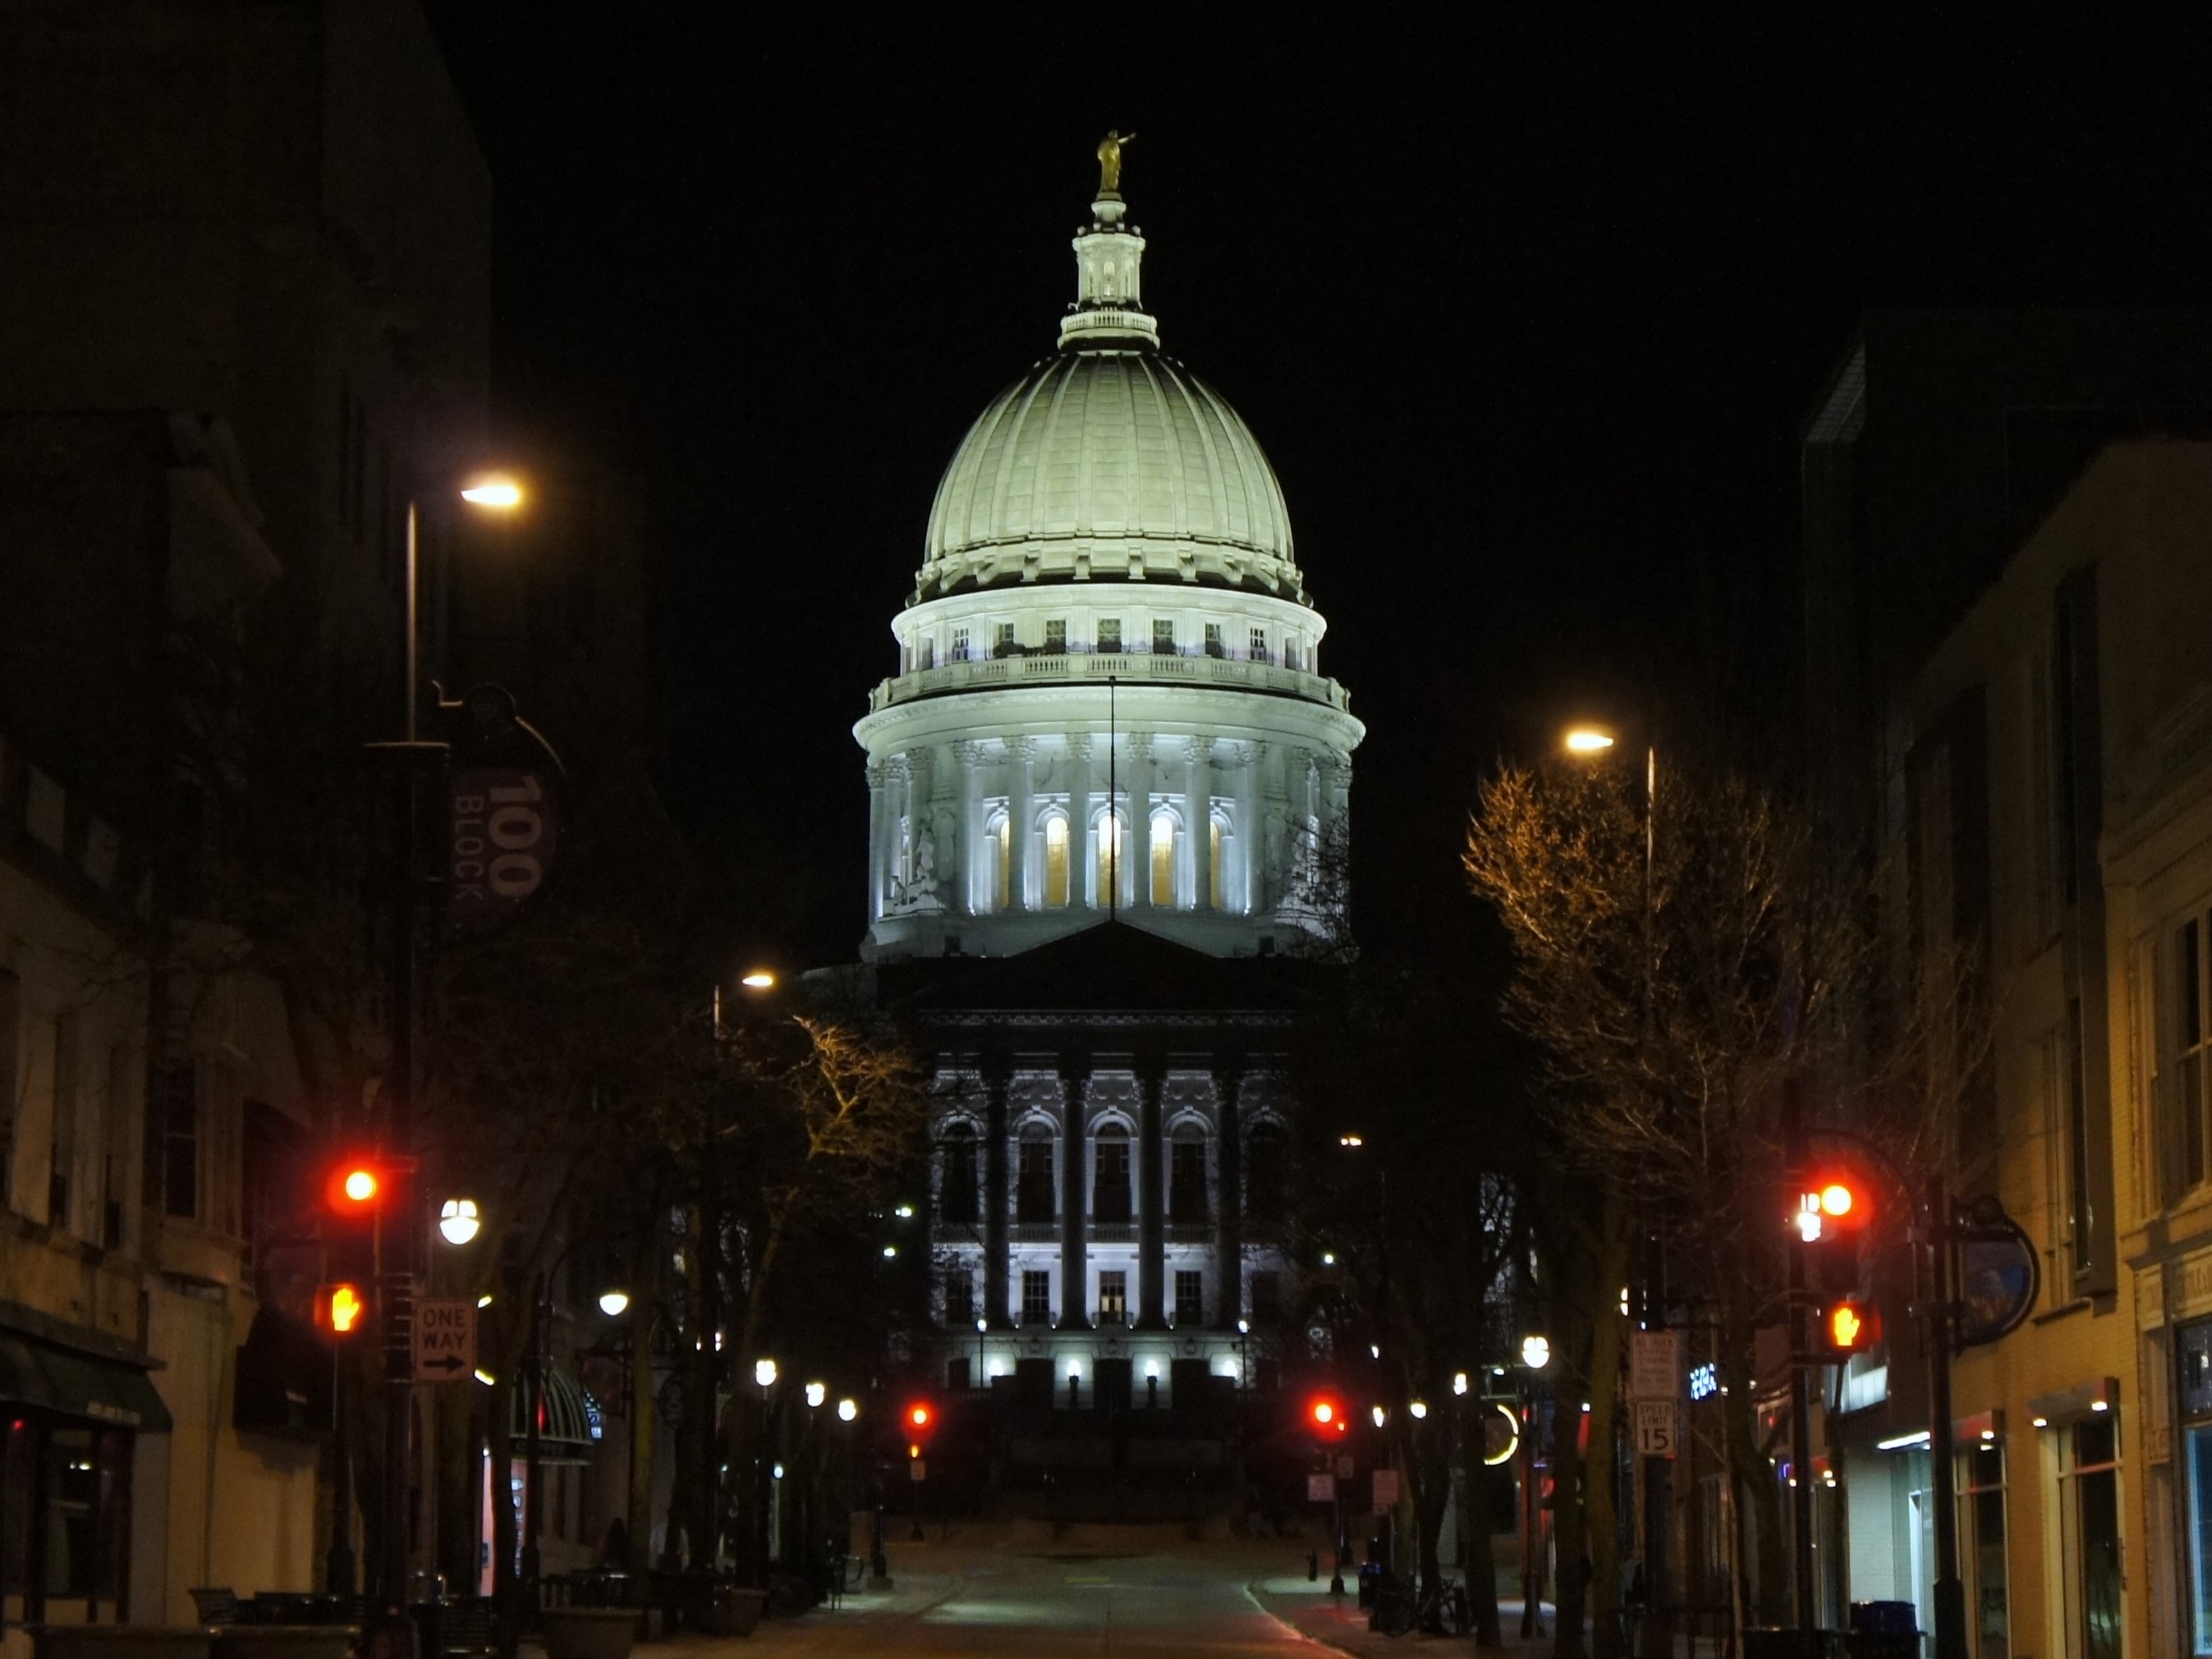
\includegraphics[scale=0.15]{DSC06893.JPG}\\
\hfill\break
Madison, the capital city of Wisconsin, one of my favorite cities in the United States.\\
Pictured in March 2024, the year I applied for my Ph.D. program. 
\end{center}

\end{document}
